\section{Architecture} % (fold)
\label{sec:architecture}
Figure \ref{fig:dependencygraph} shows the most essential parts of the internal MiCS architecture and how the parts depend on each other. 
This section will describe the different parts, how they relate to one another and how the architecture relates to the five stages outlined in section \ref{sec:workflow_overview}. 

\begin{figure}
	\begin{center}
		\centerline{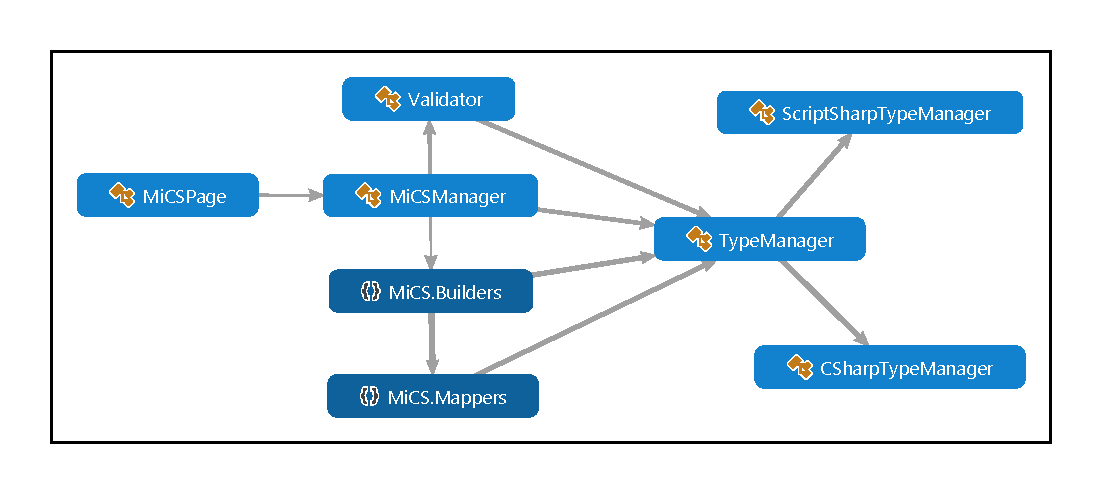
\includegraphics[width=15cm]{resources/images/architecture.pdf}}
	\end{center}
	\caption{The most important parts of the MiCS architecture.}
	\label{fig:dependencygraph}
\end{figure}


The type managers (\texttt{TypeManager}, \texttt{CSharpTypeManager} and\newline \texttt{ScriptSharpTypeManager}) provide information about types used throughout MiCS. The \texttt{CSharpTypeManager} holds information about all C\# types that can be used by the developer, including developer defined types, DOM Types and supported .NET core types. The \texttt{ScriptSharpTypeManager} only holds information about the types defined in the Script\# mscorlib.dll. The \texttt{CSharpTypeManager} and the \texttt{ScriptSharpTypeManager} each hold a semantic model (explained in section \ref{sub:microsoft_roslyn}) which is able to look up types of identifiers and expressions. By using the semantic models, the type managers are able to lookup the resultant type of an expression or the type of an identifier. The type managers are also able to determine whether a given type is developer defined type, a DOM type or a .NET core type.

The \texttt{Validator} class is responsible for validating the user's code in order to ensure correct type usage before the conversion to Script\# AST begins. The \texttt{Validator} is initiated by the MiCSManager and is dependent on the type managers.

Classes in the Builders and Mappers namespaces are responsible for converting a Roslyn AST to its corresponding Script\# AST. The Builders traverse the Roslyn AST and build a corresponding Script\# AST. The Builders are dependent on the Mappers which handle the actual conversion from Roslyn SyntaxNodes (AST nodes) to the corresponding Script\# constructs. (Stage 3)

The \texttt{MiCSManager} class ties the entire MiCS project together and is involved in all of the stages described in section \ref{sec:workflow_overview}. It initializes the TypeManagers, starts the validation, and subsequently initiates all of the processes needed to generate JavaScript. 

% % section architecture (end)